\documentclass[legalpaper,10pt]{article}
\usepackage[utf8]{inputenc}
\usepackage[activeacute,spanish]{babel}
\usepackage{amsmath, amsfonts, amssymb}
\usepackage{enumerate}
\usepackage{float}
\usepackage{indentfirst}
\usepackage{graphicx}
\usepackage{url}
\usepackage{multicol}
\usepackage{subfigure}
\usepackage[position=bottom]{subfig}
\usepackage[margin=2cm]{geometry}
% \usepackage{fullpage}
\usepackage{algorithm}
\usepackage{algorithmic}
\usepackage{caption}
% \usepackage[caption=false]{subfig}
% \setlength\parindent{0pt}
\usepackage{fancybox}

\usepackage{tikzit}
\input{sample.tikzstyles}

\begin{document}

\thispagestyle{empty}

\begin{minipage}[t]{0.6\textwidth}

{\LARGE \textbf{INF152} Estructuras Discretas}

{\large Profesores: R. Astudillo -- M. Bugueño}

Universidad Técnica Federico Santa María

Departamento de Informática -- Noviembre 10, 2020.

\end{minipage}
\hfill
\begin{minipage}[t]{0.35\textwidth}
%RELLENE CON SUS DATOS PERSONALES:
\textbf{Nombre}: Maximiliano Sepúlveda\\[0.3cm]
\textbf{Rol}: 201973536-5 \textbf{Paralelo}: 200
\end{minipage}

\vspace{0.8cm}

{\Large Certamen 2 -- Pregunta 3}

\vspace{0.4cm}

\textbf{Esta evaluación tiene como máximo 40 puntos del C2}.

\begin{enumerate}[1)]
\item Demuestre por propiedades que el grafo \(G\) de la figura posterior es bipartito. Además, demuestre o refute que existe un \emph{match} completo de los nodos que comparten coloración con el nodo \(1\) \textbf{[10 puntos]}.
\begin{center}
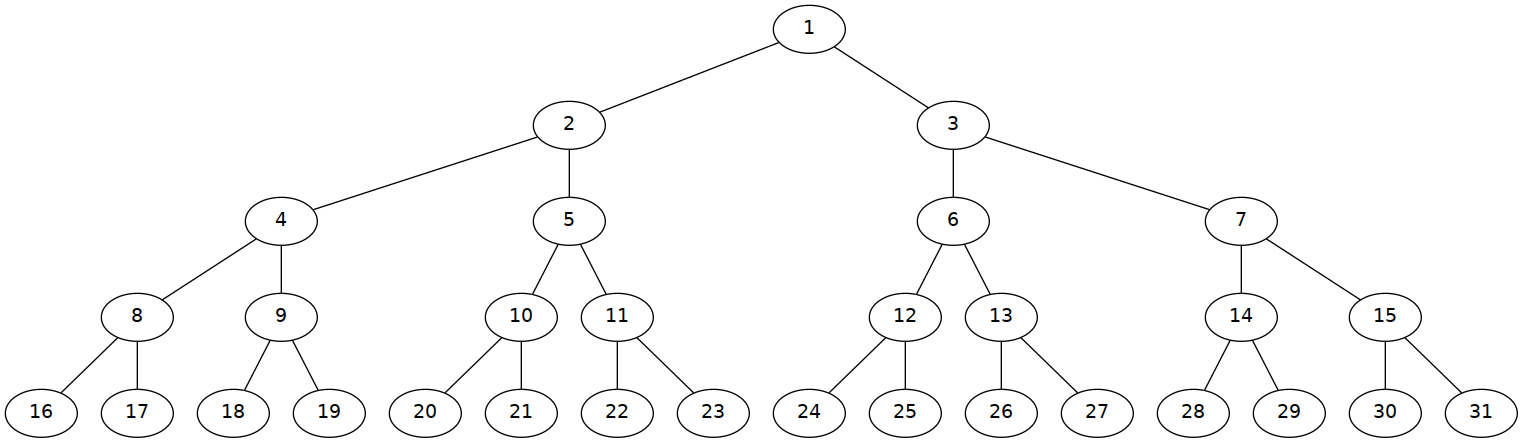
\includegraphics[scale=0.25]{./figura1.png}
\end{center}

%INDIQUE ACA SU RESPUESTA
\rule{5cm}{0.4pt}

\underline{\textbf{Respuesta:}}

Para demostrar que el grafo anterior \(G\) es bipartito, se puede utilizar el teorema que dice:
\[\boxed{\text{Un grafo es bipartito si y solo si \textbf{NO} tiene ciclos impares.}}\]

Como el grafo \(G\) es un árbol, no tiene ciclos de ningún tipo, por lo tanto, su numero cromático es 2, es decir, si es bipartito. \hfill \(\blacksquare\)

\vspace{2em}

Supongamos que el grafo se colorea, comenzando con el nodo 1 de color \textbf{azul} por ejemplo; los nodos del siguiente nivel deben ser de distinto color, \textbf{rojo} por ejemplo. Como es bipartito, solo será necesario utilizar dos colores para poder colorear todo el grafo.

Siguiendo esta idea, cada nivel del grafo quedaría coloreado de un color, y además se estarían alternando, es decir: el nivel 0 (solamente el nodo 1) quedaría coloreado de color azul, el nivel 1 (nodos 2 y 3) quedaría coloreado de color rojo, el nivel 2 (nodos 4, 5, 6 y 7) quedaría coloreado de color azul nuevamente, y así sucesivamente. Cada nivel tendrá un color alternante.

Ahora, si reorganizamos los nodos tal que tuviera forma de grafo bipartito, tendríamos los nodos azules a un lado y los rojos al otro lado. Sea el grafo de la imagen \(G = (V,E)\), consideremos entonces \(X \cup Y \subseteq V\), donde \(X\) será el conjunto de los nodos \textbf{azules}, e \(Y\) el conjunto de los nodos \textbf{rojos}. Notemos lo siguiente:
\[X = \{1,4,5,6,7,16,17,18,19,20,21,22,23,24,25,26,27,28,29,30,31\}\]
\[Y = \{2,3,8,9,10,11,12,13,14,15\}\]

El conjunto \(X\) es mucho mas grande que \(Y\). Según el teorema de Hall:

\begin{center}
  \fbox{
    \parbox{10cm}{
      Sea un grafo bipartito \(G = (X \cup Y, E)\), entonces hay un matching completo de G si, y solo si, \textbf{para cualquier} \(A \in \mathbb{P}(X)\) (es decir, \(A\) puede ser cualquier subconjunto de \(X\)) se tiene que:

      \[ |N(A)| \geq |A| \]
    }
  }
\end{center}

Para \(A\), un subconjunto de \(X\) perfectamente podría ser el trivial: el mismo conjunto \(X\). Considerando esto, es imposible que \textbf{todos} los nodos de \(A\) puedan tener matching con los nodos de \(Y\), si o si van a faltar mas nodos en \(Y\) para poder satisfacer eso.

\(\therefore\) No es posible hacer un match completo de los nodos que comparten coloración con el nodo 1. \hfill \(\blacksquare\)




\newpage






\item Sea \(G\) un grafo tal que \(\exists n \in \mathbb N,\ K_n \subseteq G\) (\(K_n\) es subgrafo de G).
  \begin{itemize}
    \item Demuestre que \( n \leq \chi (G) \) \textbf{[5 puntos]}.
    \item Determine el número cromático del siguiente grafo. Argumente su respuesta \textbf{[5 puntos]}.
      \begin{center}
        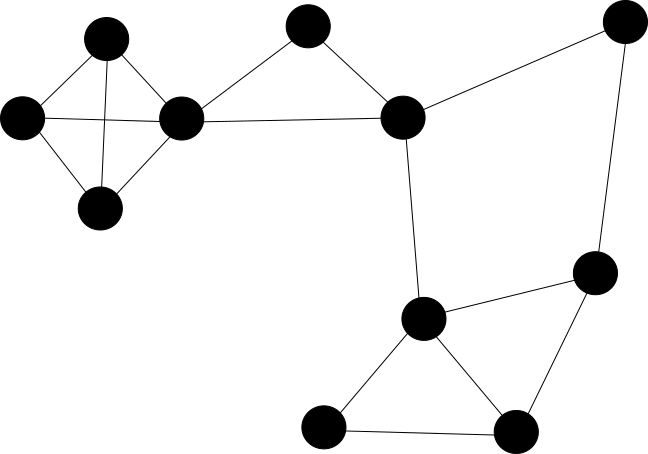
\includegraphics[scale=0.3]{./cline.png}
      \end{center}
  \end{itemize}

% INDIQUE ACA SU RESPUESTA
\rule{5cm}{0.4pt}

\underline{\textbf{Respuesta:}}

Primero comenzamos coloreando el grafo. Nos podemos fijar que hay un grafo completo de tamaño 4, esto ya nos da una pista que nos dice que hay que usar al menos 4 colores. También podemos ver ciclos de grado par e impar, pero no son mas complejos que el grafo completo anterior. Por lo tanto, su numero cromático debería ser 4.

\ctikzfig{fig1}

\[\shadowbox{\(\displaystyle \chi (G) = 4 \)}\blacksquare\]

\vspace{3em}

Debería existir un \(n\) tal que \(K_n \subseteq G\), pero como podemos ver, existen \(K_3\) dentro del grafo, y lo mas complejo que se puede encontrar es un grafo \(K_4\), en otras palabras, lo mas que puede ser \(n\) es 4.

\ctikzfig{fig2}

Y como ya vimos antes, \(\chi (G) = 4\), entonces si se cumple que \(n \leq \chi (G)\). \hfill \(\blacksquare\)



\newpage






\item Sea el grafo \(G = (X \cup Y, E)\) el grafo bipartito mostrado en la figura a continuación, con \(X = \{a \dots h\}, \ Y = \{ i \dots p \}\).
  \begin{itemize}
    \item Demuestre que la deficiencia del grafo es \textbf{al menos} 0. De tres ejemplos que corroboren que esto es así \textbf{[5 puntos]}.
    \item Utilice el algoritmo de camino alternante para encontrar el \emph{matching} maximal para el conjunto \(X\). Recuerde utilizar Tikz para mostrar su procedimiento \textbf{[15 puntos]}.
  \end{itemize}

  \begin{center}
    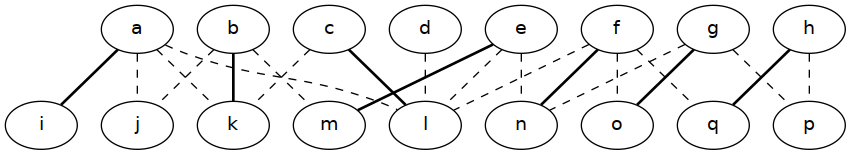
\includegraphics[scale=0.45]{./figure2.png}
  \end{center}

% INDIQUE ACA SU RESPUESTA
\rule{5cm}{0.4pt}

\underline{\textbf{Respuesta:}}

Para calcular la deficiencia del grafo, podemos usar la propiedad de:

\begin{center}
  \fbox{
    \parbox{10cm}{
      Sea \(M\) el matching maximal de un grafo bipartito \(G = (X \cup Y , E)\) con deficiencia \(d\), se cumple que:

      \[ |M| = |X| - d \]

      Se puede decir entonces que:

      \[d = |X| - |M|\]

      La deficiencia representa la cantidad de nodos que quedan fuera de un matching maximal.
    }
  }
\end{center}

Para ello podemos primero utilizar el algoritmo para poder encontrar un matching maximal:

\ctikzfig{fig3}

Podemos ver que el nodo \(d\) no tiene ningún match asociado, así que el algoritmo comienza desde ahí. El árbol que se genera es el siguiente:

\ctikzfig{fig4}

Podemos ver que hay caminos que nos llevan a ciclos. Para evitar esos caminos, podemos usar el camino que nos lleva de \(d\) hasta \(j\).


Invertir las conexiones del árbol supuestamente nos ayudara a mejorar el matching actual. Si se hace, el grafo queda de la siguiente forma:

\ctikzfig{fig5}

Como se puede ver, con el algoritmo se pudo encontrar un match maximal y completo. A consecuencia se tiene que \(|X| = 8\) y \(|M| = 8\), entonces \(\boxed{d = 0}\). Además, como es completo, no va a poder ser mejor que eso, no será menos de 0. \hfill \(\blacksquare\)

También podemos ver que en el matching maximal, no hay ningún nodo sin algún matching, esto también es una representación de que la deficiencia del grafo es 0.

En el grafo original, la deficiencia era de 1, ya que el nodo \(d\) no tenia matching. Pues, si se busca, pueden haber matching peores.







\newpage


\end{enumerate}

%RECUERDE PONER NOMBRE, ROL Y PARALELO EN EL ENCABEZADO
\end{document}
